\documentclass[10pt,journal,compsoc]{IEEEtran}
\usepackage{amsmath,amssymb}
\usepackage{booktabs}
\usepackage{array}
\usepackage{url}
\usepackage{graphicx}
\usepackage[hypertexnames=false]{hyperref}

\begin{document}

\title{Supplementary Material for ``FAIR-BETH: A Fair Thresholding and Ablation Protocol for Behavioral Malicious-Process Detection under Distribution Shift''}

\author{St\'{e}phane Ga\"{e}l R. Ekodeck \emph{et al.}}

\maketitle

\section{Feature Specification}

For process $i$, endpoint events are grouped by \texttt{hostName} and
\texttt{processId} and ordered by timestamp. The predictor excludes
\texttt{sus} and \texttt{evil}. Scalar features comprise event count, unique
event count, event entropy, argument-count mean, standard deviation and
maximum, return-value mean and standard deviation, duration, event rate,
unique argument strings, mean argument-string length, and unique parents.
The fixed event histogram is fitted on the development pool only. For event
identifier $e$,
\[
h_{i,e}=\frac{1}{n_i}\sum_{j=1}^{n_i}
\mathbf{1}\{eventId_{ij}=e\}.
\]
\[
H_i=-\sum_{e:h_{i,e}>0}h_{i,e}\log_2 h_{i,e}.
\]
The event rate is
\[
r_i=\frac{n_i}{(t_{i,n_i}-t_{i,1})+10^{-6}}.
\]
Test-only event identifiers do not expand the fitted feature space.

\section{Thresholds and Hyperparameters}

Table~\ref{tab:supp_thresholds} records the thresholds selected on
\texttt{val\_strat} for the principal ablation. Their small absolute values
must not be interpreted as deployment probabilities.

\begin{table}[t]
\centering
\caption{Validation-derived thresholds.}
\label{tab:supp_thresholds}
\begin{tabular}{lcc}
\toprule
\textbf{Model} & \textbf{5\%-FPR} & \textbf{Max-F1} \\
\midrule
IF-Platt & 0.005286 & 0.005252 \\
GRUAE-Platt & 0.005408 & 0.005129 \\
SimpleAvg & 0.005318 & 0.005190 \\
ScoreRF & 0.059149 & 0.088814 \\
TabRF & 0.018254 & 0.174148 \\
MetaRF & 0.016541 & 0.195849 \\
\bottomrule
\end{tabular}
\end{table}

\begin{table}[t]
\centering
\caption{Principal model hyperparameters.}
\label{tab:supp_hyperparameters}
\begin{tabular}{lll}
\toprule
\textbf{Component} & \textbf{Parameter} & \textbf{Value} \\
\midrule
Isolation Forest & Trees & 200 \\
Isolation Forest & Contamination & 0.0050 \\
GRU-AE & Embedding/hidden & 32/64 \\
GRU-AE & Layers/parameters & 1/42\,482 \\
GRU-AE & Batch size/epochs & 512/30 \\
GRU-AE & Learning rate & $10^{-3}$ \\
ScoreRF & Trees/minimum leaf & 200/2 \\
TabRF & Trees/input dimensions & 200/61 \\
MetaRF & Trees/input dimensions & 300/64 \\
RF-500 & Trees/class weights & 500/balanced \\
Bootstrap & Replicates & 1\,000 \\
\bottomrule
\end{tabular}
\end{table}

The sequence capacity audit uses the first 512 tokens, batch size 128, Adam
with learning rate $10^{-3}$, at most eight epochs, and patience two. It
predicts token $t+1$ from tokens through $t$; the target token is never fed to
the decoder at the same position. The three tested configurations are
GRU-64$\times$1 (23\,666 parameters), GRU-128$\times$2 (183\,218), and
LSTM-128$\times$2 (241\,074).

\section{Repeated Threshold Procedure}

The enriched development pool combines the training, calibration, and
stratified-validation partitions and contains 5\,819 processes, including 29
positives. Repeated stratified five-fold validation with ten repetitions
produces 50 held-out score vectors. Each fold contains five or six positives.
An RF-500 model is fitted independently in each fold and the largest-recall
threshold satisfying empirical validation FPR $\leq0.05$ is stored. The median
threshold is computed before any official-test evaluation. A final RF-500 is
then fitted on the full development pool and evaluated once with the locked
median threshold. Test-label access is not part of model fitting, threshold
selection, or aggregation. Table~\ref{tab:supp_threshold_sensitivity} reports
the resulting sensitivity across all preselected thresholds.

\begin{table}[t]
\centering
\caption{Sensitivity over all 50 preselected thresholds on the fixed test score vector.}
\label{tab:supp_threshold_sensitivity}
\begin{tabular}{lccc}
\toprule
\textbf{Metric} & \textbf{Median} & \textbf{Minimum} & \textbf{Maximum} \\
\midrule
Precision & 0.7573 & 0.7411 & 0.7979 \\
Recall & 0.6446 & 0.6198 & 0.6860 \\
F1 & 0.6964 & 0.6964 & 0.7124 \\
Observed FPR & 0.3247 & 0.2468 & 0.3766 \\
False positives & 25 & 19 & 29 \\
False negatives & 43 & 38 & 46 \\
\bottomrule
\end{tabular}
\end{table}

\section{Reproducibility Checklist}

The executable order is: read the public BETH CSV files; exclude DNS files;
aggregate by host and process; derive labels; remove label fields; fit the
event vocabulary on development data; construct scalar, histogram, and
sequence representations; create train, calibration, and validation
partitions; train detectors and baselines; fit score calibration on calibration
data; lock thresholds on validation data; evaluate the official test once; and
write CSV, JSON, score, and figure artifacts. The repeated-threshold and
sequence-capacity scripts are independent audits and do not overwrite the
principal artifacts.

Authoritative generated files include
\texttt{cross\_fitted\_thresholds.csv},
\texttt{locked\_threshold\_test\_sensitivity.csv},
\texttt{sequence\_capacity\_ablation.csv}, and their JSON summaries. The
complete package is available at
\url{https://github.com/EkodeckStephane/fair-beth-malicious-process-detection}.

\section{Data and Model Cards}

\textbf{Data purpose:} offline evaluation of behavioral malicious-process
detection under distribution shift. BETH is not a complete representation of
production ransomware and lacks family labels. Supplementary BETH files are
development data only; the official test remains the final BETH test.
MalBehavD-V1 validates protocol portability to another schema, not direct
transfer of a BETH-trained model.

\textbf{Model purpose:} the direct tabular forests are research benchmarks,
not endpoint products. They use observable process statistics and event
histograms. Their main limitation is threshold non-transfer: a 5\% development
FPR becomes 32.47\% for the repeated-validation locked threshold and 36.36\%
for TabRF's principal threshold on the official test.

\textbf{Failure disclosure:} anomaly-score ranking inverts; score fusion does
not beat the direct tabular baseline; recurrent next-event variants remain
weak; early BETH prefixes provide low recall; calibration scores have no
reliable posterior interpretation under test shift; host-disjoint threshold
selection is unstable; and the official BETH test contains only 198 processes.

\section{Supplementary Audit Figures}

Figure~\ref{fig:supp_reliability} provides the calibration curves,
Figures~\ref{fig:supp_malbehavd_importance} and
\ref{fig:supp_beth_importance} report held-out permutation attribution, and
Figure~\ref{fig:supp_beth_prefix} reports the BETH prefix curve.

\begin{figure*}[t]
\centering
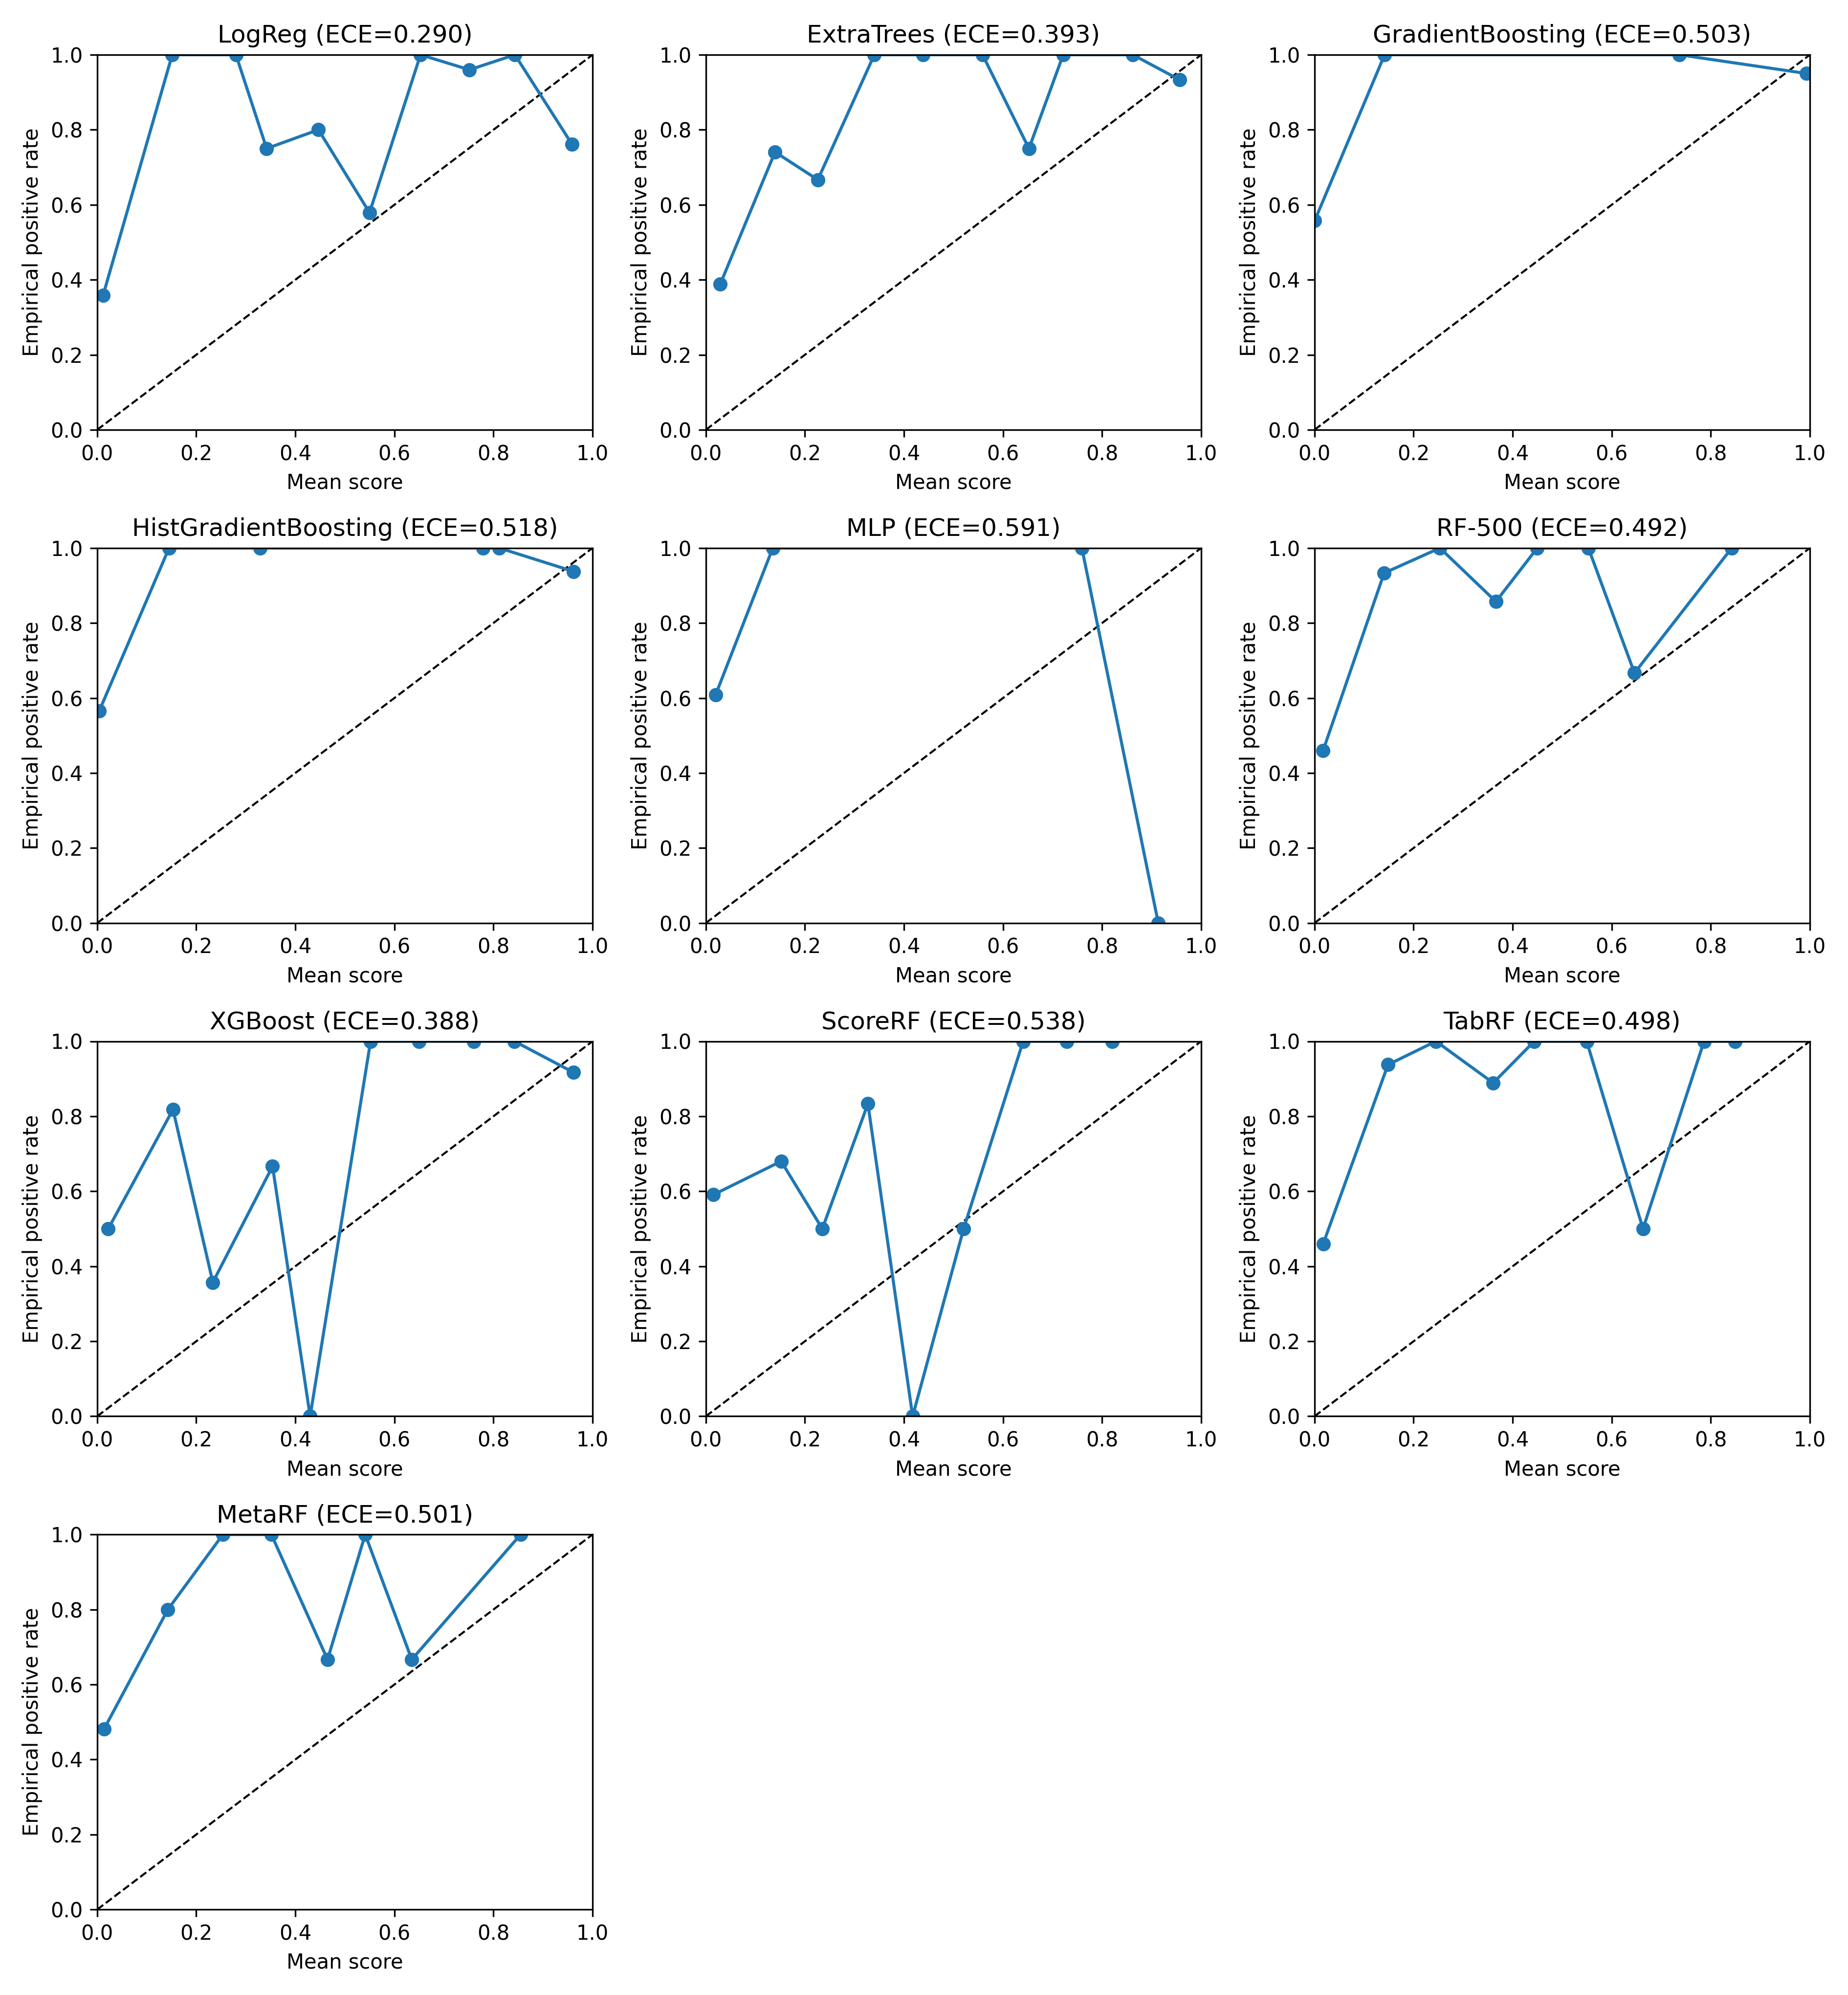
\includegraphics[width=0.94\textwidth]{reliability_diagrams.png}
\caption{Reliability diagrams on the official BETH test split. These curves support score-and-threshold language rather than posterior-risk language.}
\label{fig:supp_reliability}
\end{figure*}

\begin{figure}[t]
\centering
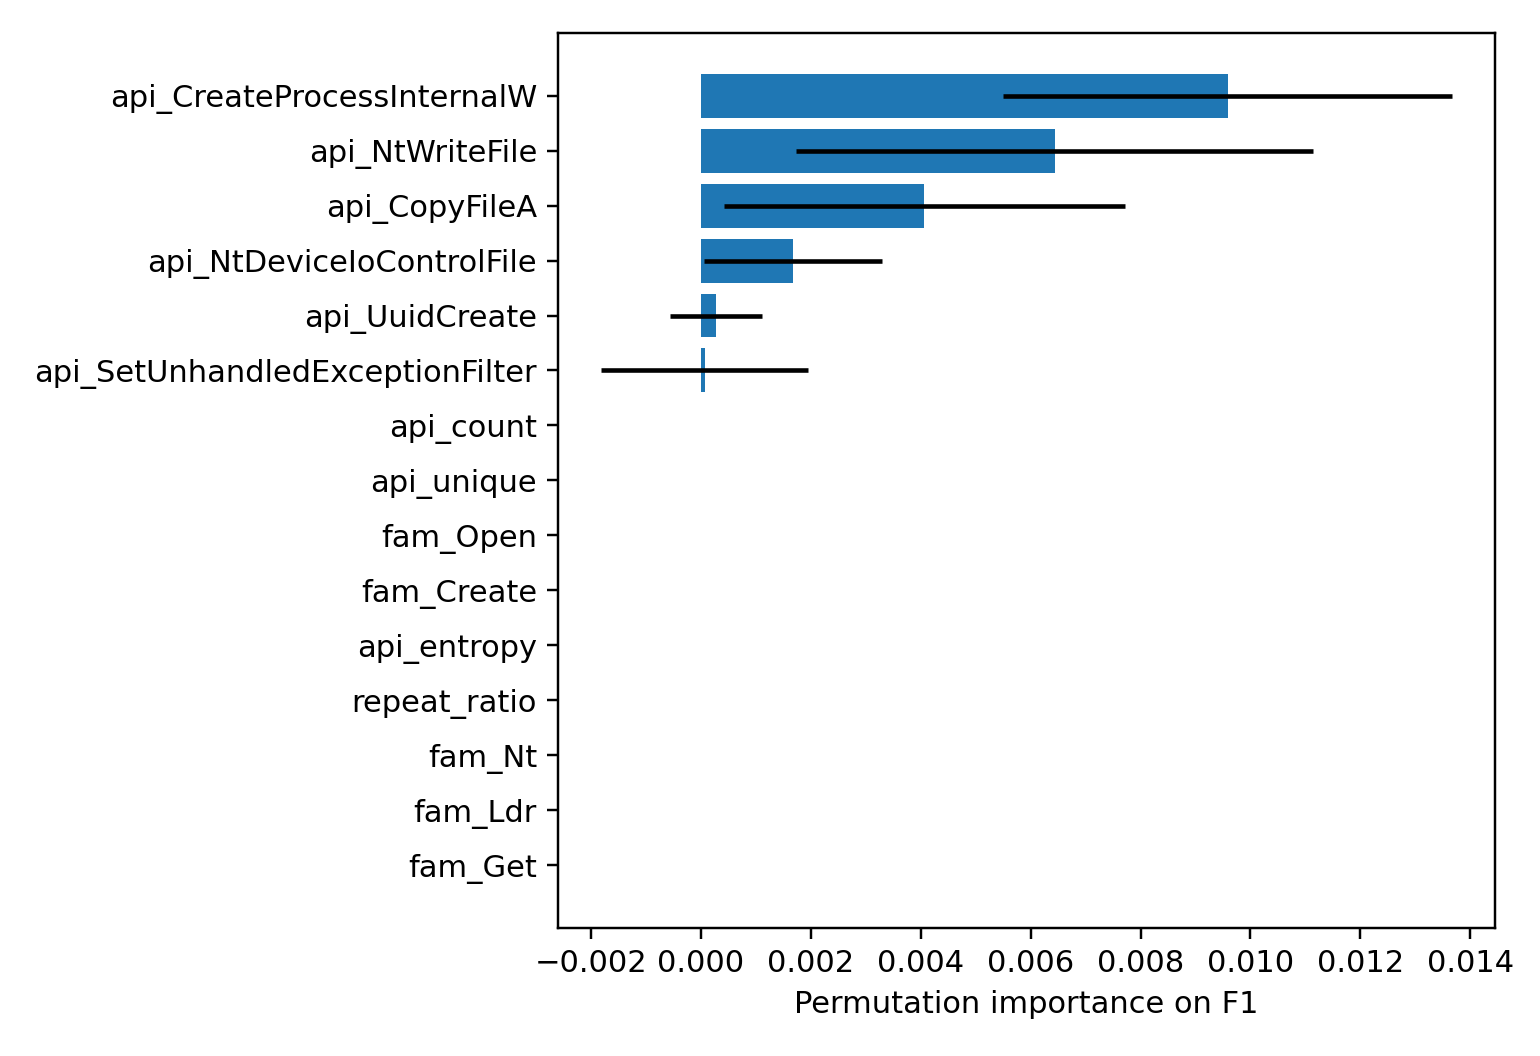
\includegraphics[width=0.95\linewidth]{malbehavd_feature_importance.png}
\caption{Held-out permutation importance on MalBehavD-V1.}
\label{fig:supp_malbehavd_importance}
\end{figure}

\begin{figure}[t]
\centering
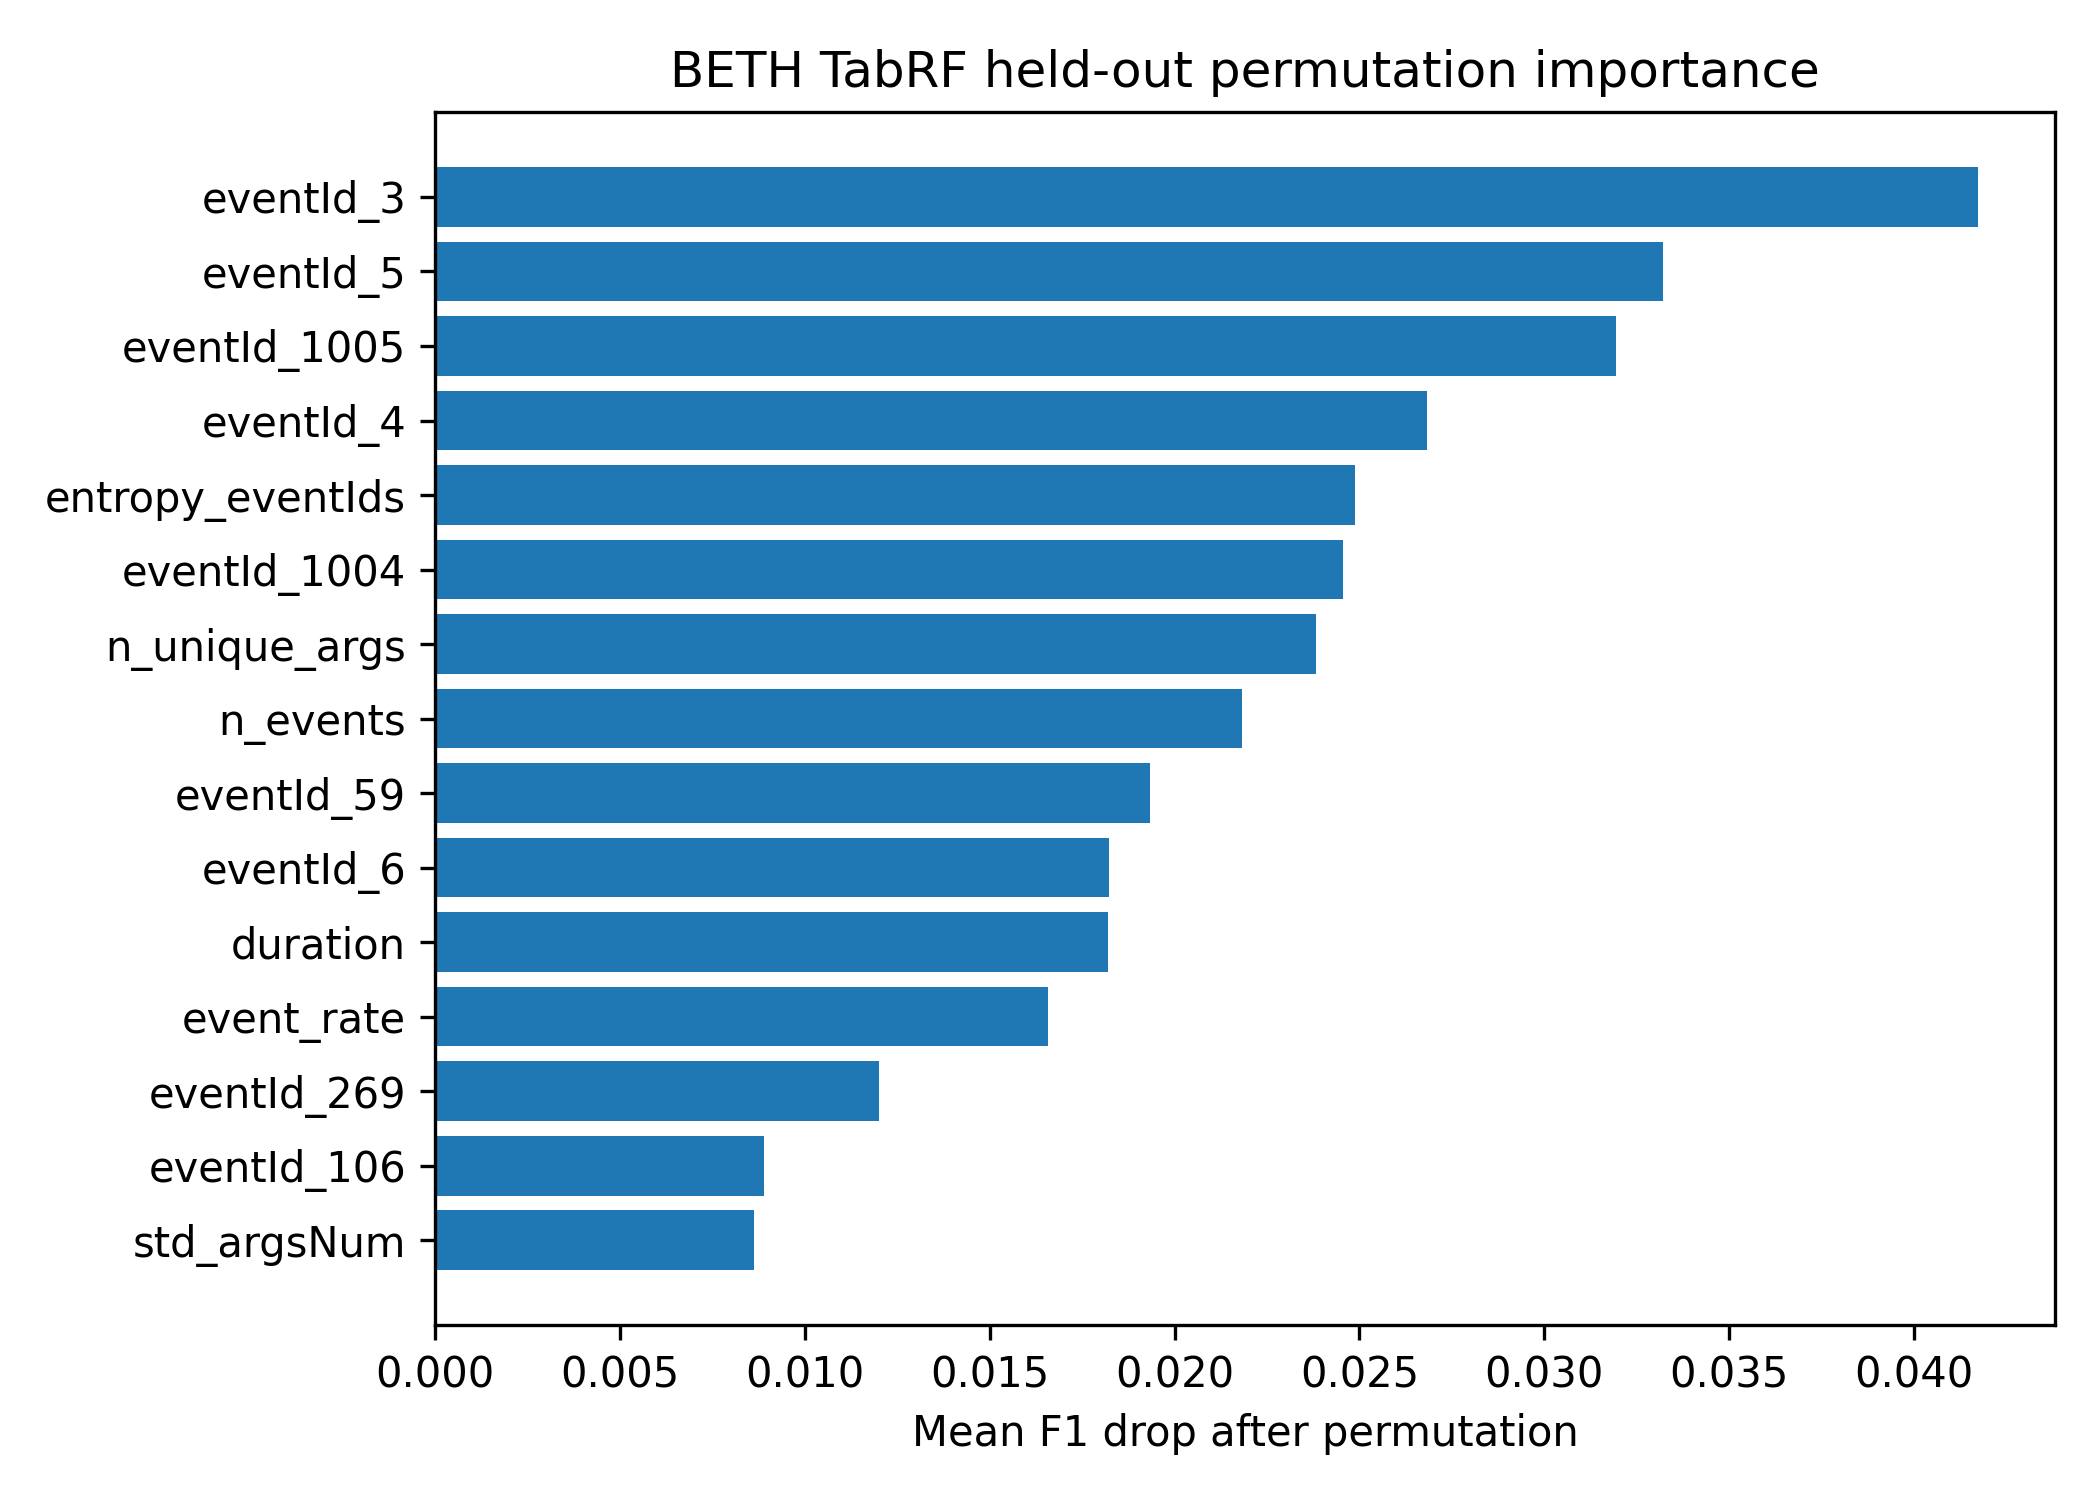
\includegraphics[width=0.95\linewidth]{beth_tabrf_permutation_importance.png}
\caption{Held-out permutation importance for BETH TabRF.}
\label{fig:supp_beth_importance}
\end{figure}

\begin{figure}[t]
\centering
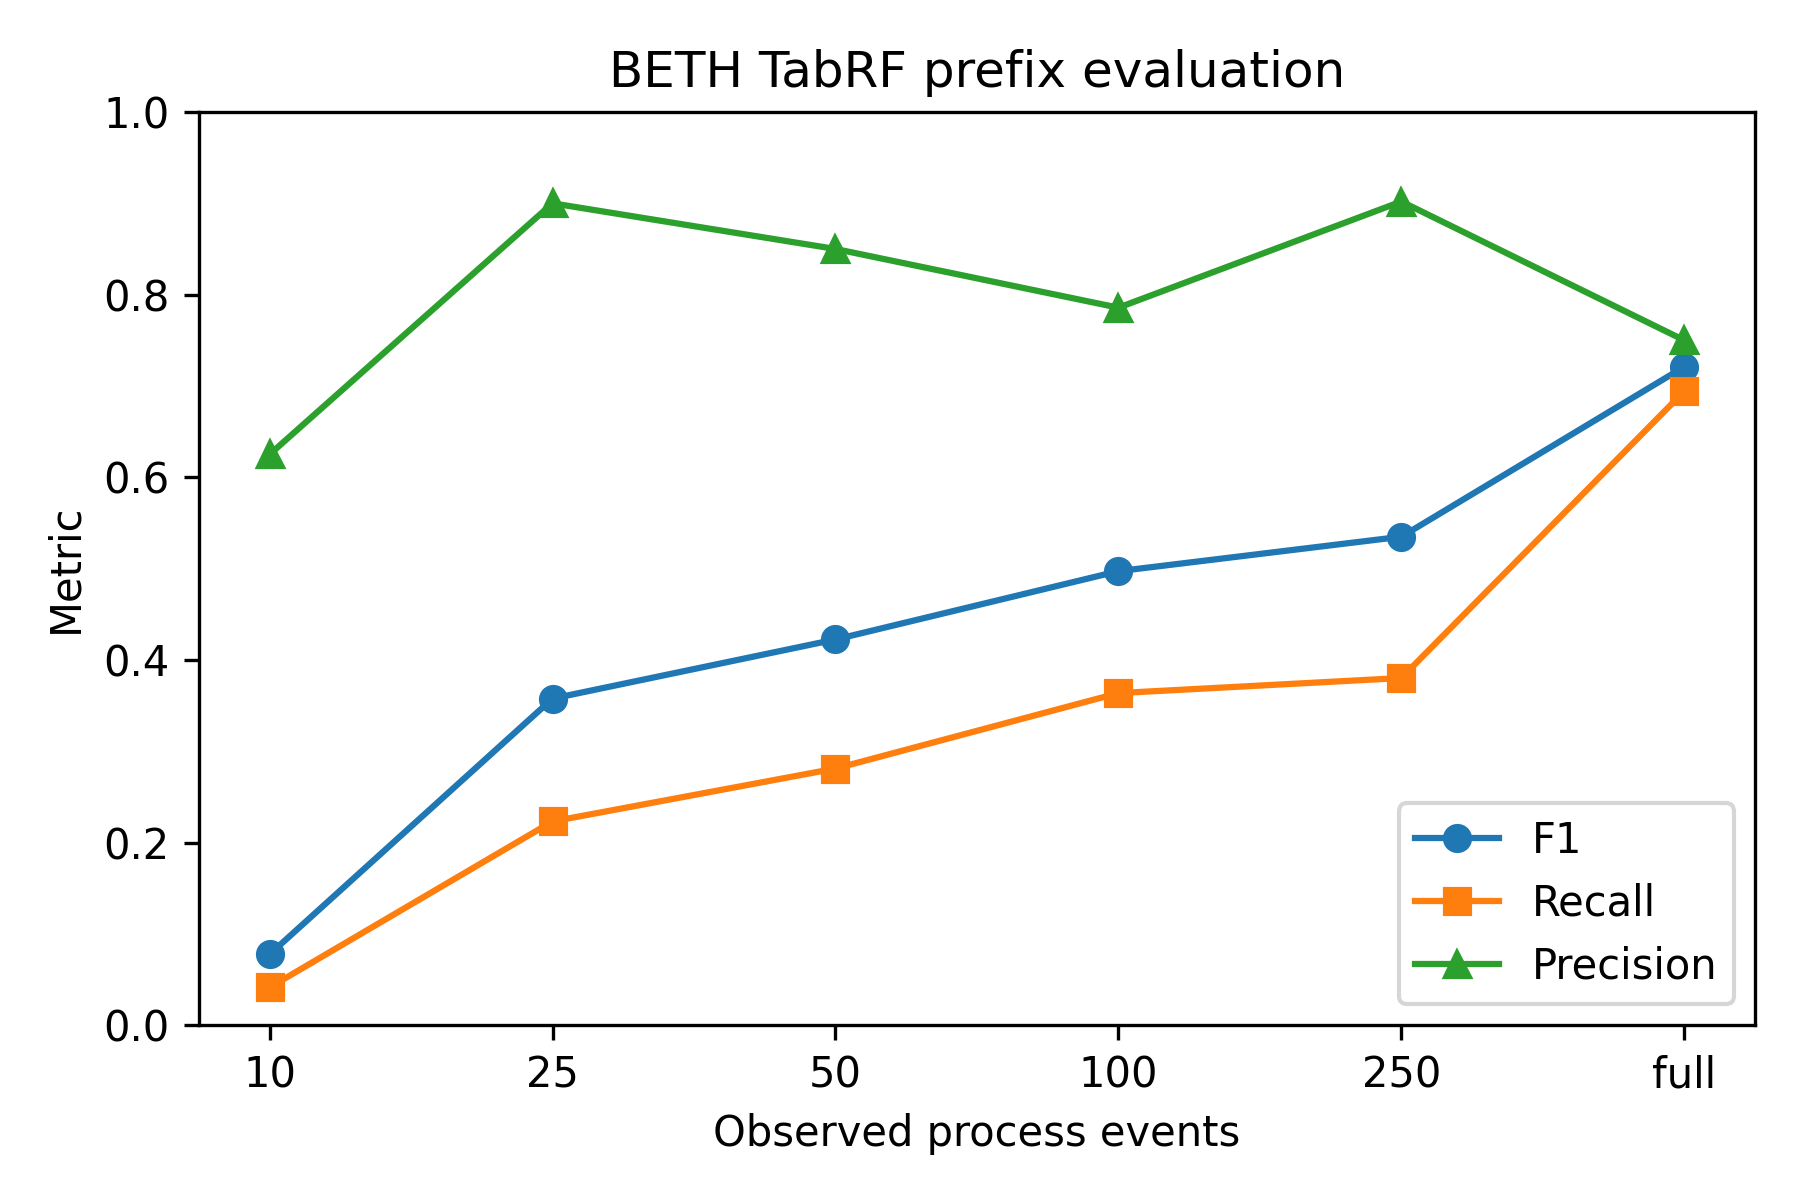
\includegraphics[width=0.95\linewidth]{beth_prefix_curve.png}
\caption{BETH TabRF prefix evaluation.}
\label{fig:supp_beth_prefix}
\end{figure}

\section{Deployment and Response Boundary}

A live implementation must maintain rolling state per process and recompute
features over prefixes. The paper's full-trace result cannot establish
containment latency. Thresholds require target-environment calibration,
host-role stratification, drift monitoring, and reversible response policies.
Suggested actions range from evidence collection to network constraint; process
termination requires corroborating signals and rollback safeguards. MITRE
ATT\&CK may organize analyst response, but BETH event identifiers are not used
as technique labels because the dataset does not supply a validated mapping.

\section{Extension Requirements}

Direct transfer requires a schema-compatible endpoint dataset with benign and
malicious processes, host and time metadata, and enough positive processes for
independent calibration and testing. Family-specific claims additionally
require verified family labels. A complete deployment study must report
wall-clock detection delay, replay-based evasion, action reversibility, analyst
workload, and predeclared cost functions. Oracle test thresholds may be shown
only as sensitivity analyses and must never replace the locked operating point.

\end{document}
